%!TEX root = thesis.tex

\chapter{Proposed architecture}
\label{chapter:Proposed architecture}

Based on the aspects pointed out on Chapter~\ref{chapter:Payment terminal acceptance testing}, this part of the master's thesis will present a proposed architecture for automated acceptance testing environment for payment terminal software. Components of the environment can be divided into hardware and software components and this chapter is divided accordingly.

Research done in this master's thesis was carried out in co-operation with Eficode Oy and one of its customers providing payment terminal software in the Nordic countries. Motivation for this project came from the customer and Eficode Oy took responsibility of implementing the system according to the best practices of the industry. This proposal was initial plan for the project and it will be presented in this chapter.

\section{Overview}

When planning an automated acceptance test (AAC) environment for payment terminal software, environment has to be highly adaptive for different types of hardware and software features of different payment terminal models. This proposal was done for one payment terminal software provider and they had several different models of payment terminals and altogether 51 different software configurations for those devices.

Security is a top priority of payment terminal electronics and software and it is not possible to access internals of the payment terminal hardware. This means that AAC environment has to be able to manipulate the physical interface of the device. This also creates requirement for supporting different types of keyboard layouts and screen locations. In other words, environment has to be non dependent on single manufacturer or payment terminal model.

One of the requirements for the AAC environment was also use of open source technologies. For the reasons pointed out in Section~\ref{section:Open source}, customer wanted that the environment is as open as possible. This also creates reputation and visibility regarding the security matters.

Other requirements for the AAC environment was simplicity, low cost, low need for maintenance and ability to run the tests 24/7.

\section{Hardware}
\label{section:Proposed hardware}

Hardware for this proposal was intendedly kept simple and low-cost as possible. This proposal presents the use of just one Raspberry Pi 2\footnote{\url{https://www.raspberrypi.org/products/raspberry-pi-2-model-b/}} computer as a main computer for AAC environment. Raspberry Pi 2 in relatively inexpensive compared to its computing power and it can also run full Linux operating system. It is small sized and does not require any cooling equipment. Therefore it suites well to this project as it can be situated easily to the environment and can be run over the clock without concerns about wearing cooling fans for example.

AAC environment also requires computer vision as changes on the screen have to observed. Manufacturer of Raspberry Pi offers low-price solution for this as a form of Raspberry Pi Camera Module\footnote{\url{https://www.raspberrypi.org/products/camera-module/}}. This module is proposed for use in computer vision tasks of the AAC environment.

\FloatBarrier
\subsection{The Robot}

To be able to manipulate the physical UI of the payment terminals, some sort of robot is needed. Robot should be therefore able to accommodate different types of payment terminals and be able to press all types of buttons in question. Low cost and low need for maintenance are also requirements for this robot.

The master's thesis proposes the use of ShapeOko 2\footnote{\url{http://www.shapeoko.com/wiki/index.php/ShapeOko_2}} Computer Numerical Control (CNC) milling machine to be used as a manipulator. Though the machine is intended for milling purposes, it can be turned into a portal robot when milling tool is removed.

ShapeOko 2 is an open-source project and plans of the machine are openly available on their GitHub\footnote{\url{https://github.com/shapeoko/Shapeoko_2}}. This allows easy modifications to the hardware parts of the robot if needed.

ShapeOko 2 has a working area of about 300 mm x 300 mm x 60 mm and this meas that it can accommodate up to three payment terminals at same time to the working area. This allows parallel test case execution i.e. test cases can be run at the same time with different terminals.

ShapeOko 2 is controlled by an Arduino board running a program called GRBL. GRBL is an open source, high performance G-code interpreter and it is used for controlling CNC milling machines in general\footnote{\url{http://www.shapeoko.com/wiki/index.php/Software}}. G-code command are sent from Raspberry Pi 2 to the Arduino on the robot using serial communication.

Robot should be equipped with a pushing tool that can be manipulate the buttons. Pushing tool can be easily manufactured using for example 3D printing techniques.

\FloatBarrier
\subsection{Card Feeder}

Insertion and removal of the credit card might be hard to accomplish in a simple way using just the robot described in previous section. This work proposes the use of generally designed card feeders to accomplish this task. Proposed card feeders consist of 3D printed base plate that attaches to the payment terminal, servo motor and 3D printed tray that attaches to the servo and to the credit card.

Card feeders are designed in a way that they can be used with any types payment terminals that have the card slot at the bottom edge of the device. Standard hobby servos are used as servo motors in order to keep the cost of the setup low.

Arduino board will be used to drive the servos as it can easily provide the needed pulse width modulated (PWM) signal for the servos. Raspberry Pi on the machine will communicate with Arduino through serial communication.

\section{Software}

For software part of this AAC environment, Raspbian Wheezy is proposed for operating system. Raspbian is the official supported operating system by the Raspberry Pi Foundation\footnote{\url{https://www.raspberrypi.org/downloads/raspbian/}}. Raspbian is based on widely used Debian Unix-like operating system. This allows the use of components developed for Debian to be used with this AAC environment.

As different keyboard layouts have to be supported, some kind of configuration files are proposed. There should be two types of configuration files: one for device locations in the working area of the robot and one for each keyboard layout. In this way configuration of devices under test can be easily modified at test case level.

\FloatBarrier
\subsection{Test Framework}

Robot Framework\footnote{\url{http://robotframework.org/}} is proposed for the test framework. RF is an open-source, generic, keyword-driven test automation framework that has human readable test case syntax (\emph{\cite{Rfuserguide}}).

Robot Framework also has highly modular software architecture (\emph{\cite{Rfuserguide}}) and this allows the framework to be used with any kinds of testing libraries to connect to the system under test. This feature can be seen as a great advantage when implementing test libraries for machine control and computer vision (Chapter~\ref{subsection:test libraries}). Illustration of this modular architecture can be seen in Figure~\ref{fig:modular_architecture} bellow.

\begin{figure}[ht]
  \begin{center}
    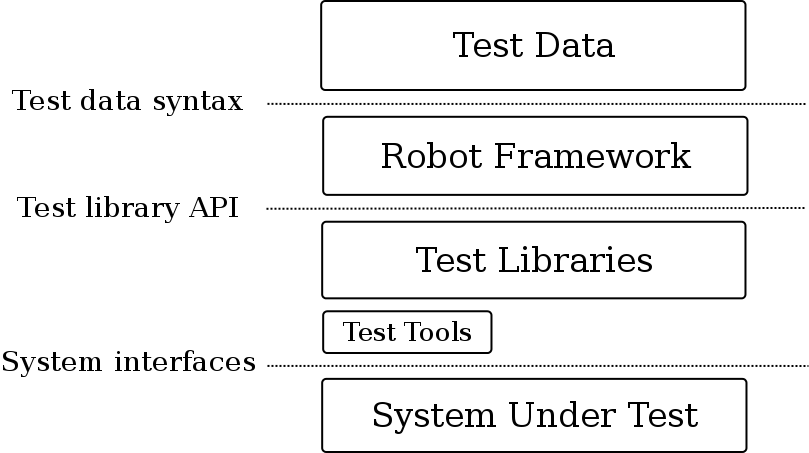
\includegraphics[width=8cm]{images/architecture-big.png}
    \caption{High level modular architecture. Source: \url{http://robotframework.org/img/architecture-big.png}}
    \label{fig:modular_architecture}
  \end{center}
\end{figure}

When RF tests are being run, it generates clear report and log files of the test case execution results (\emph{\cite{Rfuserguide}}). These files offer high level view of all test cases and step-by-step descriptions of individual test cases in order to make the debugging more easy.

Example of intended test case can be seen in Figure~\ref{fig:invalid_pin_test}. This test case describes automated RF acceptance test for entering invalid PIN code when trying to execute card purchase.

\begin{figure}[ht]
  \begin{center}
    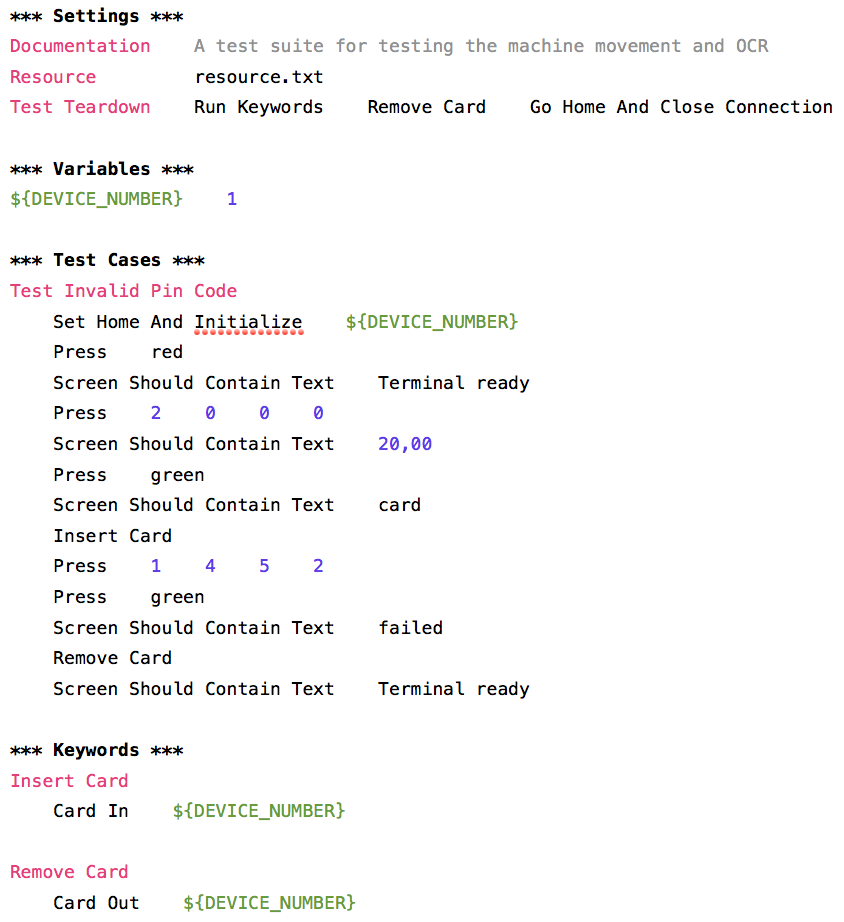
\includegraphics[width=10cm]{images/example_test.png}
    \caption{Example test case for invalid PIN code test}
    \label{fig:invalid_pin_test}
  \end{center}
\end{figure}

\FloatBarrier
\subsection{Test Libraries}
\label{subsection:test libraries}

As can be seen on Figure~\ref{fig:modular_architecture}, architecture requires external libraries to connect to the system under test. In this case those libraries would be a library for machine control, a library for computer vision and a library for card feeder manipulation. All these libraries can be written using Python programming language that is supported out of the box by Robot Framework (\emph{\cite{robotframework}}).

For machine control library the environment has to be able to send G-code command through USB serial communication to Arduino on the robot. For this pySerial\footnote{\url{http://pythonhosted.org/pyserial/}} library is proposed.

For the computer vision task of the environment, messages on the display are usually those that need to be verified. For this character recognition is needed. Open source optical character recognition (OCR) engine called Tesseract OCR\footnote{\url{https://github.com/tesseract-ocr/tesseract}} is proposed. It was initially developed by HP but since 2006 it has been developed by Google. In order to use Tesseract OCR with Python, pytesseract\footnote{\url{https://pypi.python.org/pypi/pytesseract}} wrapper is needed.

Library for controlling the card feeders is the most simplest one of these three libraries. For this pySerial\footnote{\url{http://pythonhosted.org/pyserial/}} library is proposed to send the serial communication command to the Arduino controlling the card feeders.